\section{Phương pháp}

\subsection{Vì sao không forecast observed sales trực tiếp?}

Observed sales là biến có thể bị censor bởi tồn kho. Trong giờ stockout, doanh số quan sát được là phần bán được trước khi hết hàng hoặc bằng không, không nhất thiết bằng demand thật. Nếu train model trực tiếp trên observed sales, mô hình có thể học rằng các chuỗi thường hết hàng có demand thấp. Điều này dẫn đến under-forecast và quyết định replenishment thiếu hàng.

\subsection{Two-stage framework}

Pipeline chính gồm hai stage. Stage 1 recover latent demand ở cấp hourly cho các giờ stockout. Stage 2 aggregate hourly recovered demand lên daily và forecast tổng nhu cầu 7 ngày tiếp theo. Cách này giữ thông tin stockout chi tiết ở nơi nó xuất hiện, nhưng trả forecast cuối ở cấp daily phù hợp hơn cho quyết định vận hành.


\begin{figure}[H]
    \centering
    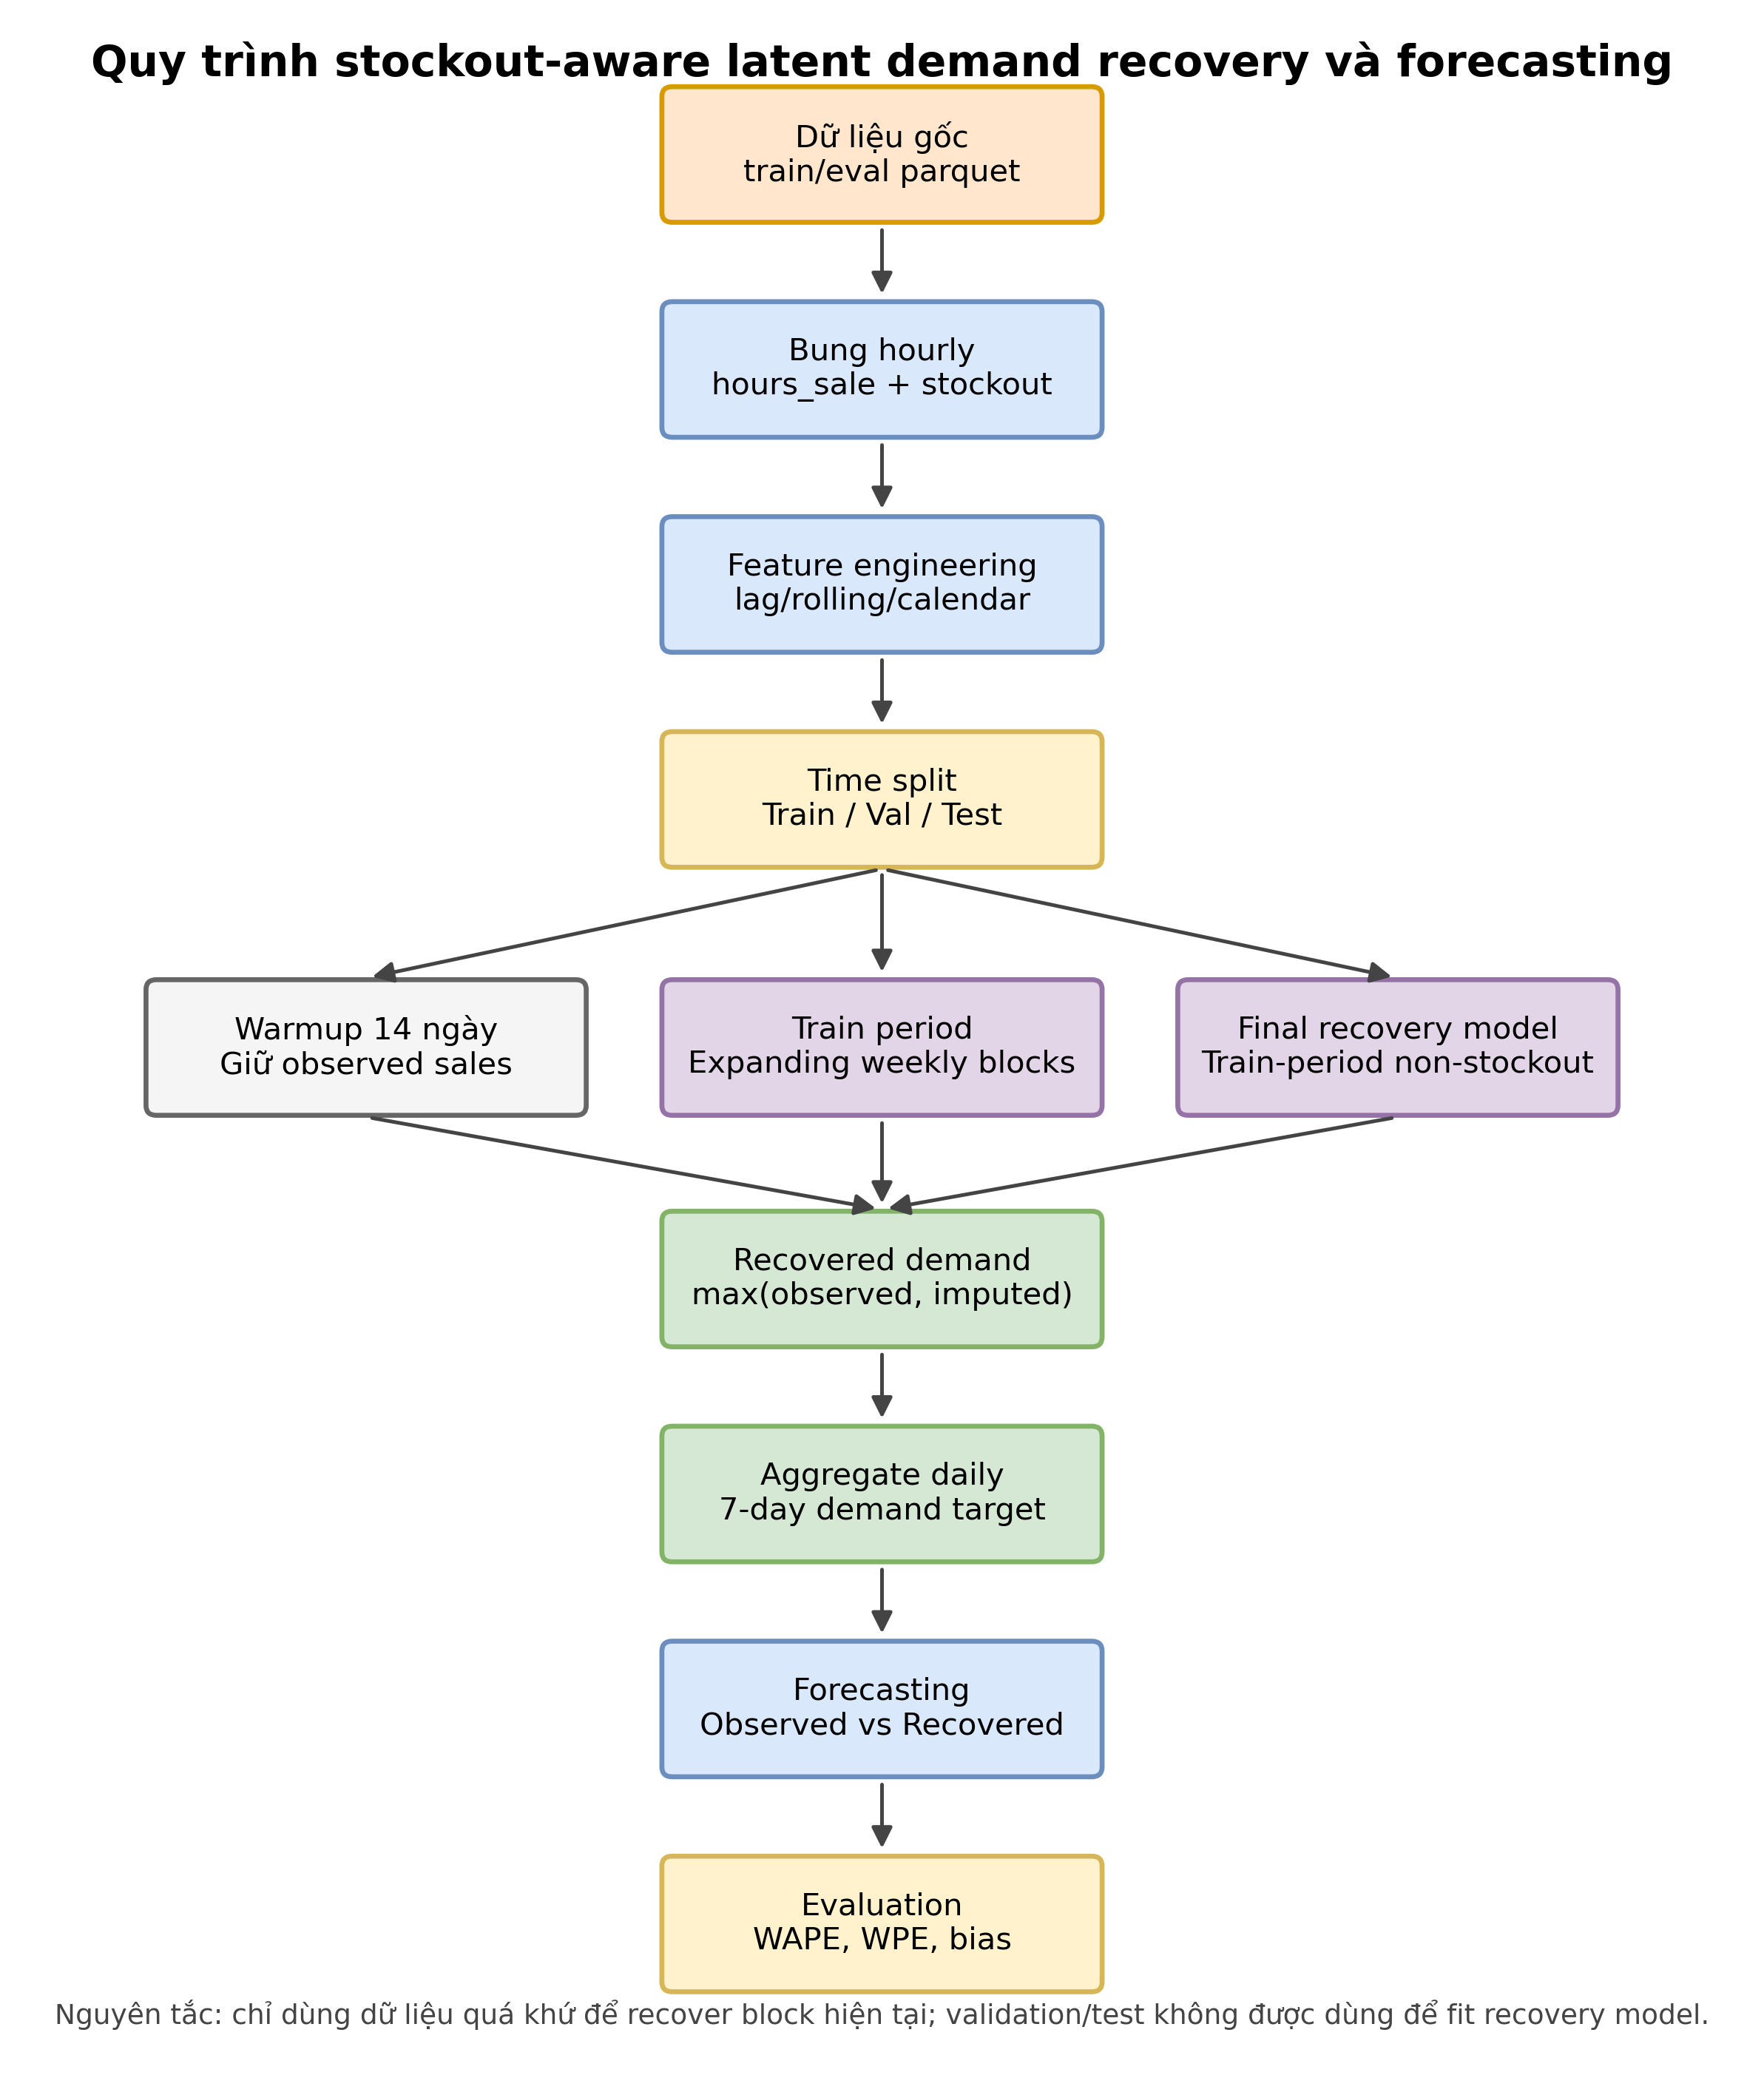
\includegraphics[width=0.88\linewidth]{figures/owner_expanding_window_process.png}
    \caption{Quy trình tổng quát two-stage.}
    \label{fig:long-process}
\end{figure}


\subsection{Expanding-window recovery}

Điểm dễ gây leakage nhất là latent demand recovery. Nếu dùng dữ liệu tương lai để impute quá khứ, forecast sau đó sẽ quá lạc quan. Vì vậy, trong train period, recovery được thực hiện theo block 7 ngày: mỗi block chỉ được recover bằng model học từ non-stockout rows nằm trước block đó. Validation/test được recover bằng final recovery model train trên non-stockout rows của train period.


\begin{figure}[H]
    \centering
    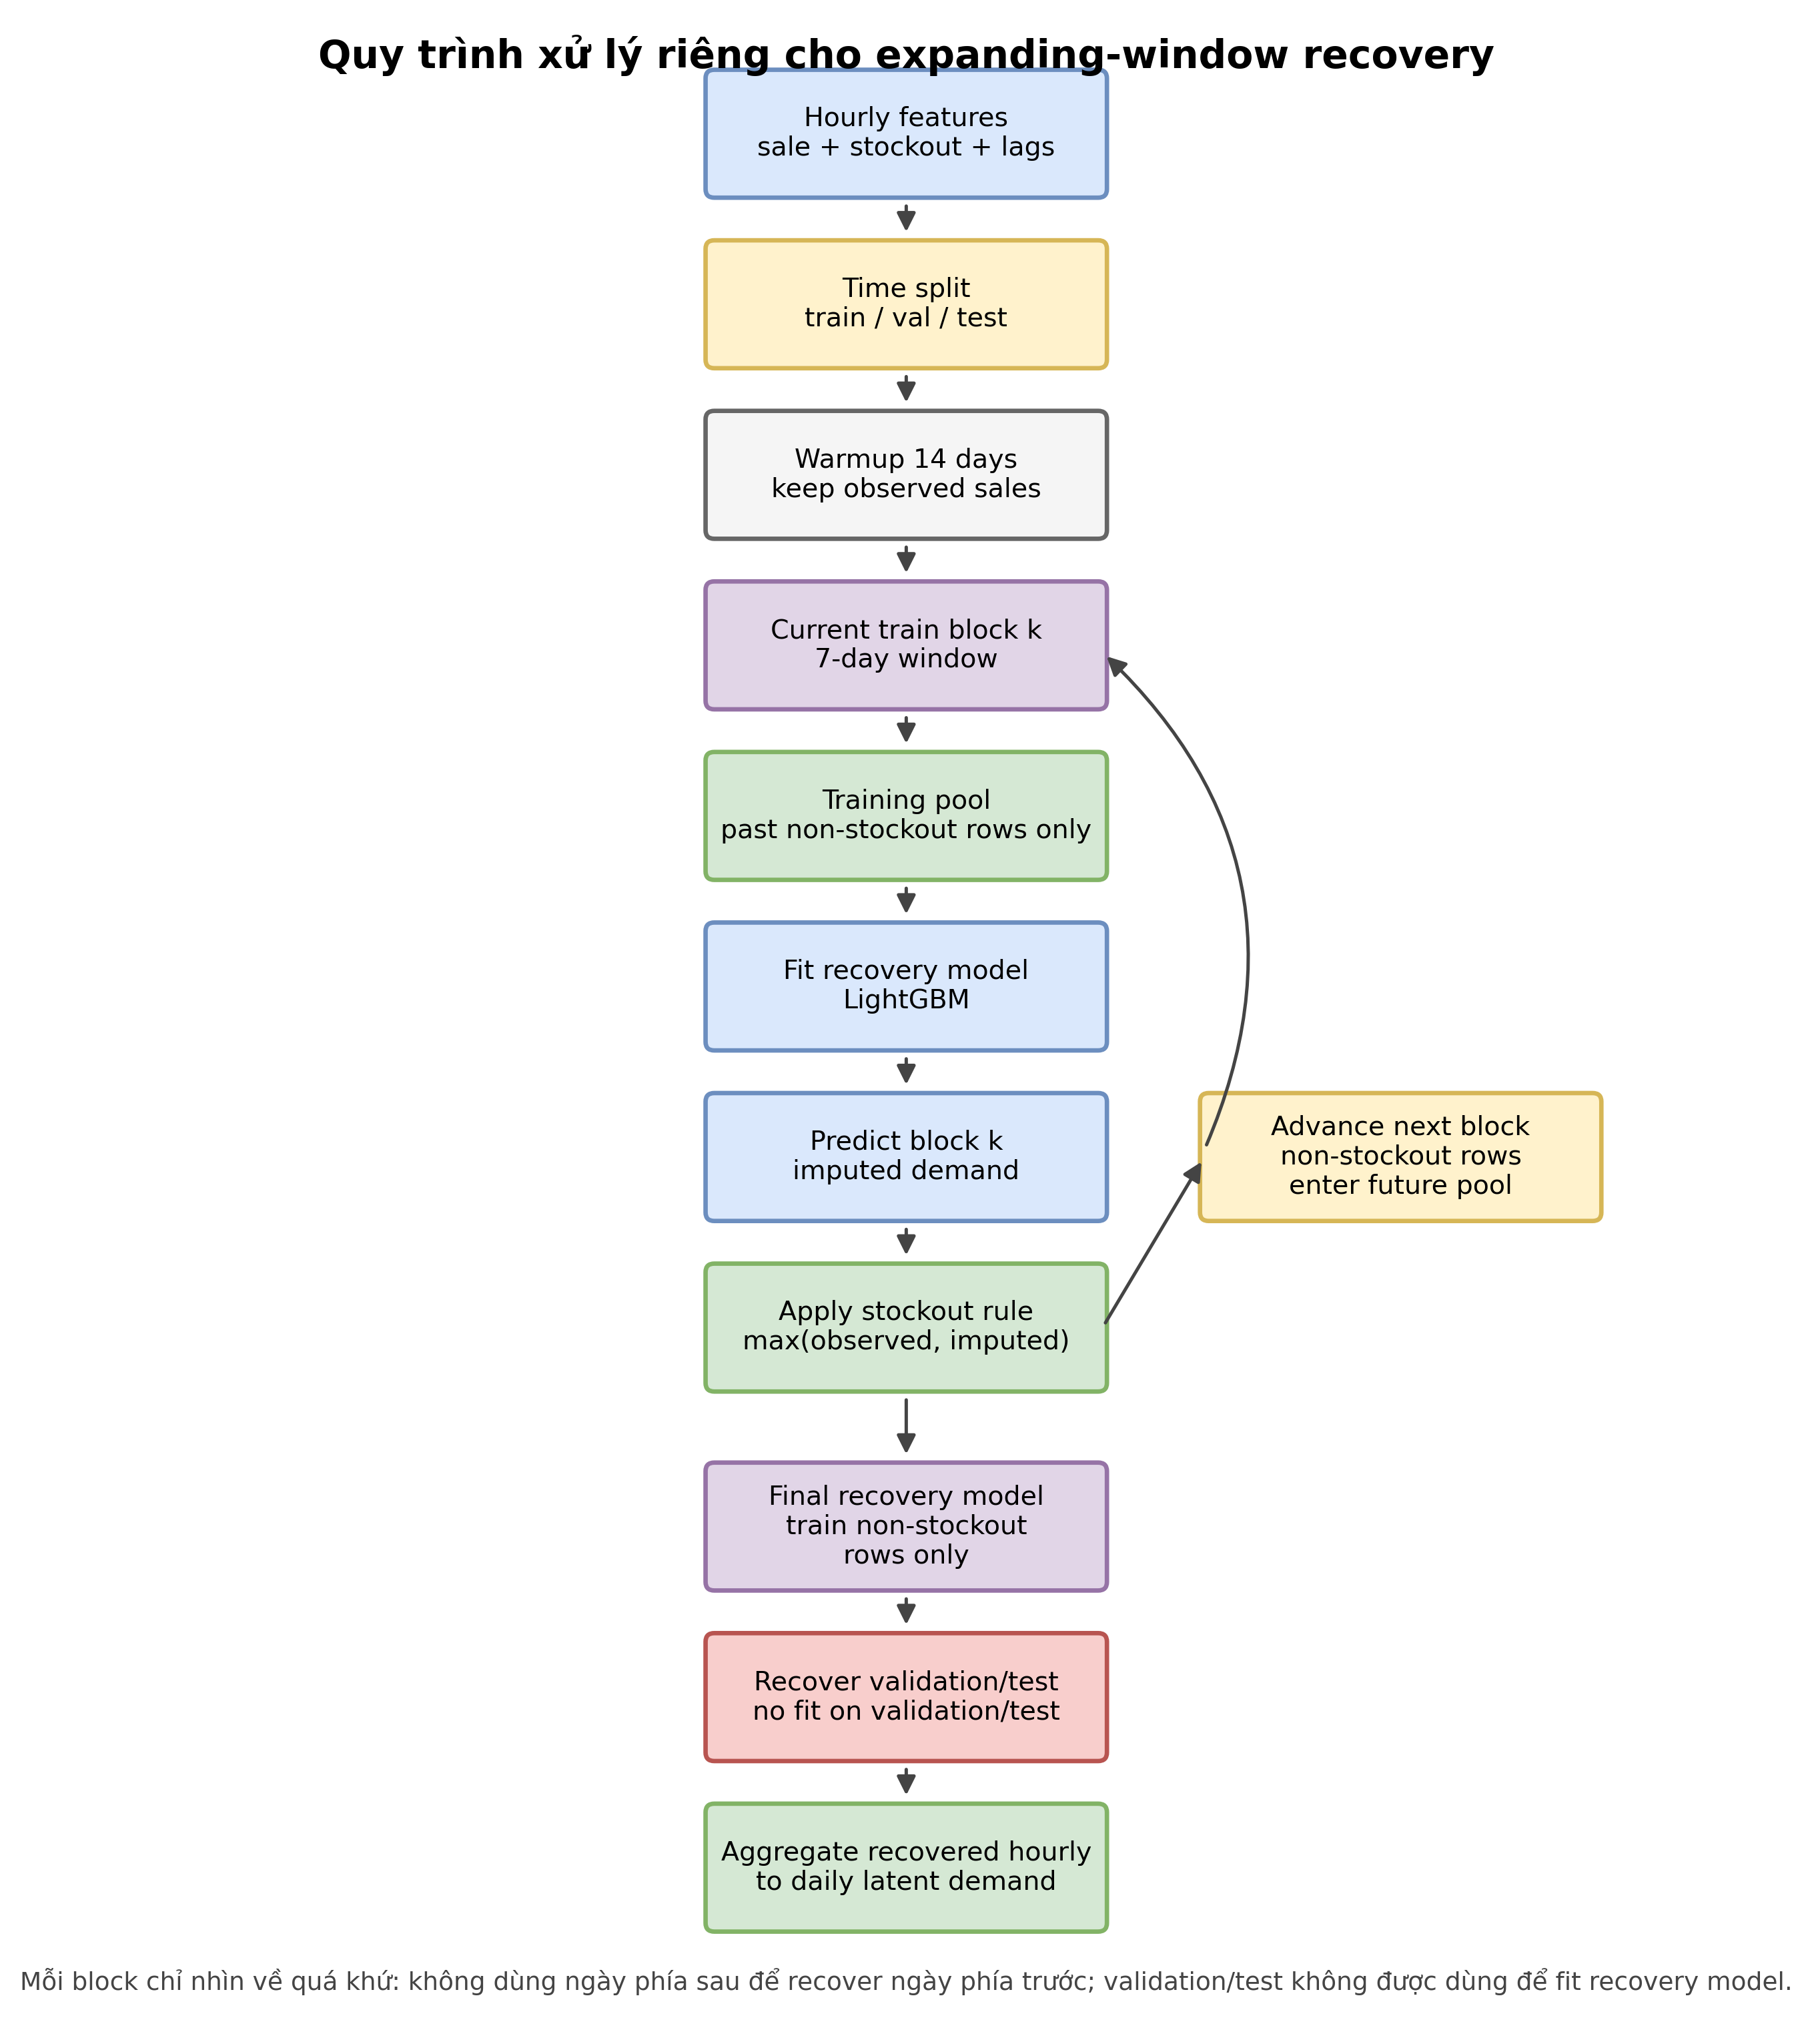
\includegraphics[width=0.90\linewidth]{figures/owner_expanding_window_recovery_detail.png}
    \caption{Chi tiết expanding-window recovery.}
    \label{fig:long-recovery-detail}
\end{figure}


\subsection{Calibration và cap}

Raw imputed demand có thể overpredict. Do đó, dự đoán raw được hiệu chỉnh bằng calibration factor học từ validation non-stockout rows. Sau đó lost demand dương được cap ở q90 để tránh một số giờ stockout cực trị làm tổng demand tăng quá mức. Công thức triển khai là:

\[
\text{lost}_t = \max\left(\frac{\hat{y}^{raw}_t}{c} - y^{obs}_t, 0\right),
\quad
\text{lost}^{cap}_t = \min(\text{lost}_t, q90),
\quad
y^{rec}_t = y^{obs}_t + \text{lost}^{cap}_t.
\]

\subsection{Daily forecasting target}

Sau recovery hourly, dữ liệu được aggregate lên daily. Target chính là \texttt{target\_next7\_recovered\_daily}, tức tổng recovered demand trong 7 ngày sau forecast origin. Target dạng tổng 7 ngày phù hợp với bài toán replenishment hơn forecast từng giờ riêng lẻ vì quyết định nhập hàng thường dựa trên nhu cầu vài ngày tới.

\subsection{Modeling choice}

LightGBM được chọn vì đây là bài toán tabular time-series quy mô lớn với nhiều feature lag, rolling, calendar, stockout, promotion và weather. Classical ARIMA/SARIMA không được chọn làm model chính vì khó scale tới hàng nghìn chuỗi store-product và khó xử lý chuỗi thưa. Deep learning không phải trọng tâm vì yêu cầu tuning/tài nguyên cao hơn, trong khi mục tiêu đồ án là một pipeline có thể giải thích và tái lập.

\subsection{Baselines và hybrid}

Báo cáo không chỉ so sánh hai mô hình ML. Các baseline daily gồm naive x7, seasonal naive 7-day và rolling mean 14-day. Seasonal naive 7-day rất mạnh do dữ liệu có seasonality tuần rõ. Vì vậy, mô hình cuối là hybrid seasonal-ML: blend giữa seasonal naive 7-day và recovered-demand LightGBM, với trọng số chọn trên validation set.
